\section{Eksperyment}
\subsection{Laser krawędziowy 635\,nm (L635P003) --- omówienie wyników}
Pomiar przeprowadzony był w temperaturach chłodnicy od 278\,K do 308\,K, z krokiem co 5\,K. Wartości wyznaczonego prądu progowego
znajdują się w tabeli~\ref{tab:tabela_635}. Rysunki od ~\ref{fig:plot_i_th_4} do ~\ref{fig:plot_eff_via_current_all} dotyczą lasera
krawędziowego 635\,nm.
\begin{itemize}
\item Wykres na rysunku~\ref{fig:plot_i_th_4} przedstawia sposób wyznaczana wartość prądu progowego. Następnie na podstawie
wyznaczonych wartości w danej temperaturze, sporządziłem wykres prądu progowego w zależności od temperatury
przedstawiony na rysunku~\ref{fig:plot_fit}. Do wykreślonych wartości punktów dopasowałem funkcję~\ref{eq:i_th} w wyniku otrzymałem
 temperaturą charakterystyczną $T_0$, która wynosiła ($47 \pm 2$)\,K oraz parametr $I_0$ o wartości (0.05 $\pm$ 0.02)\,mA
\item Analizując wykres napięcia na laserze od prądu wejściowego przedstawiony na rysunku~\ref{fig:plot_voltage_power_635}
można zauważyć, że wraz ze wzrostem temperatury na chłodnicy
maleje opór lasera. Wraz z wyższą temperaturą chłodnicy maleje także moc wyjściowa lasera.
\item Wykres na rysunku~\ref{fig:plot_eff_via_current4_635} przedstawia sprawność różniczkowa lasera w funkcji prądu wejściowego
w różnych temperaturach chłodnicy. W górnej części rysunku pokazana jest zależność mocy wyjściowej od prądu, do której dopasowałem
funkcją kwadratową dla punktów leżących powyżej wartości prądu progowego. Dopasowana funkcja zbliżona jest do funkcji liniowej, przez co sprawność różniczkowa jest
prawie stała, jednakże jak wynika z wykresu im wyższa temperatura tym sprawność lasera mniejsza, aczkolwiek zmiany na
przestrzeni są małe około 0.010\,W/A.
\item Wykres na rysunku~\ref{fig:plot_eff_via_current_all} przedstawia jak zmienia się sprawność lasera od temperatury chłodnicy.
Funkcje, które przedstawiają sprawność zostały wyznaczone analogicznie jak te przedstawione na rysunku~\ref{fig:plot_eff_via_current4_635}.
Analizując ten wykres, dochodzę do wniosku, że wraz ze wzrostem temperaturą sprawność różniczkowa lasera maleje.
\end{itemize}
\begin{table}[H]
\begin{center}
\caption{Wyznaczone wartośc prądu progowego $I_{\mathrm{th}}$ w różnych temperaturach $T$ dla lasera krawędziowego 635\,nm. }
\begin{tabular}{ | C{1.5cm}|  C{1.5cm} | C{1.5cm} | C{1.5cm}| C{1.5cm} | C{1.5cm}| C{1.5cm}| C{2.0cm}| C{2.0cm}|}
\hline
$T$ [K] 	&   278 & 283  	& 288 & 293 & 298 & 303 & 308 \\ \hline
$I_{\mathrm{th}}$ [mA]  &	19.1 $\pm$ 0.2  & 20.7 $\pm$ 0.2 & 22.6 $\pm$ 0.2 &
25.0 $\pm$ 0.2  & 27.9 $\pm$ 0.3 & 31.4 $\pm$ 0.5 & 36 $\pm$ 2	\\ \hline
\end{tabular}
\label{tab:tabela_635}
\end{center}
\end{table}
%\begin{figure}
%\center
%  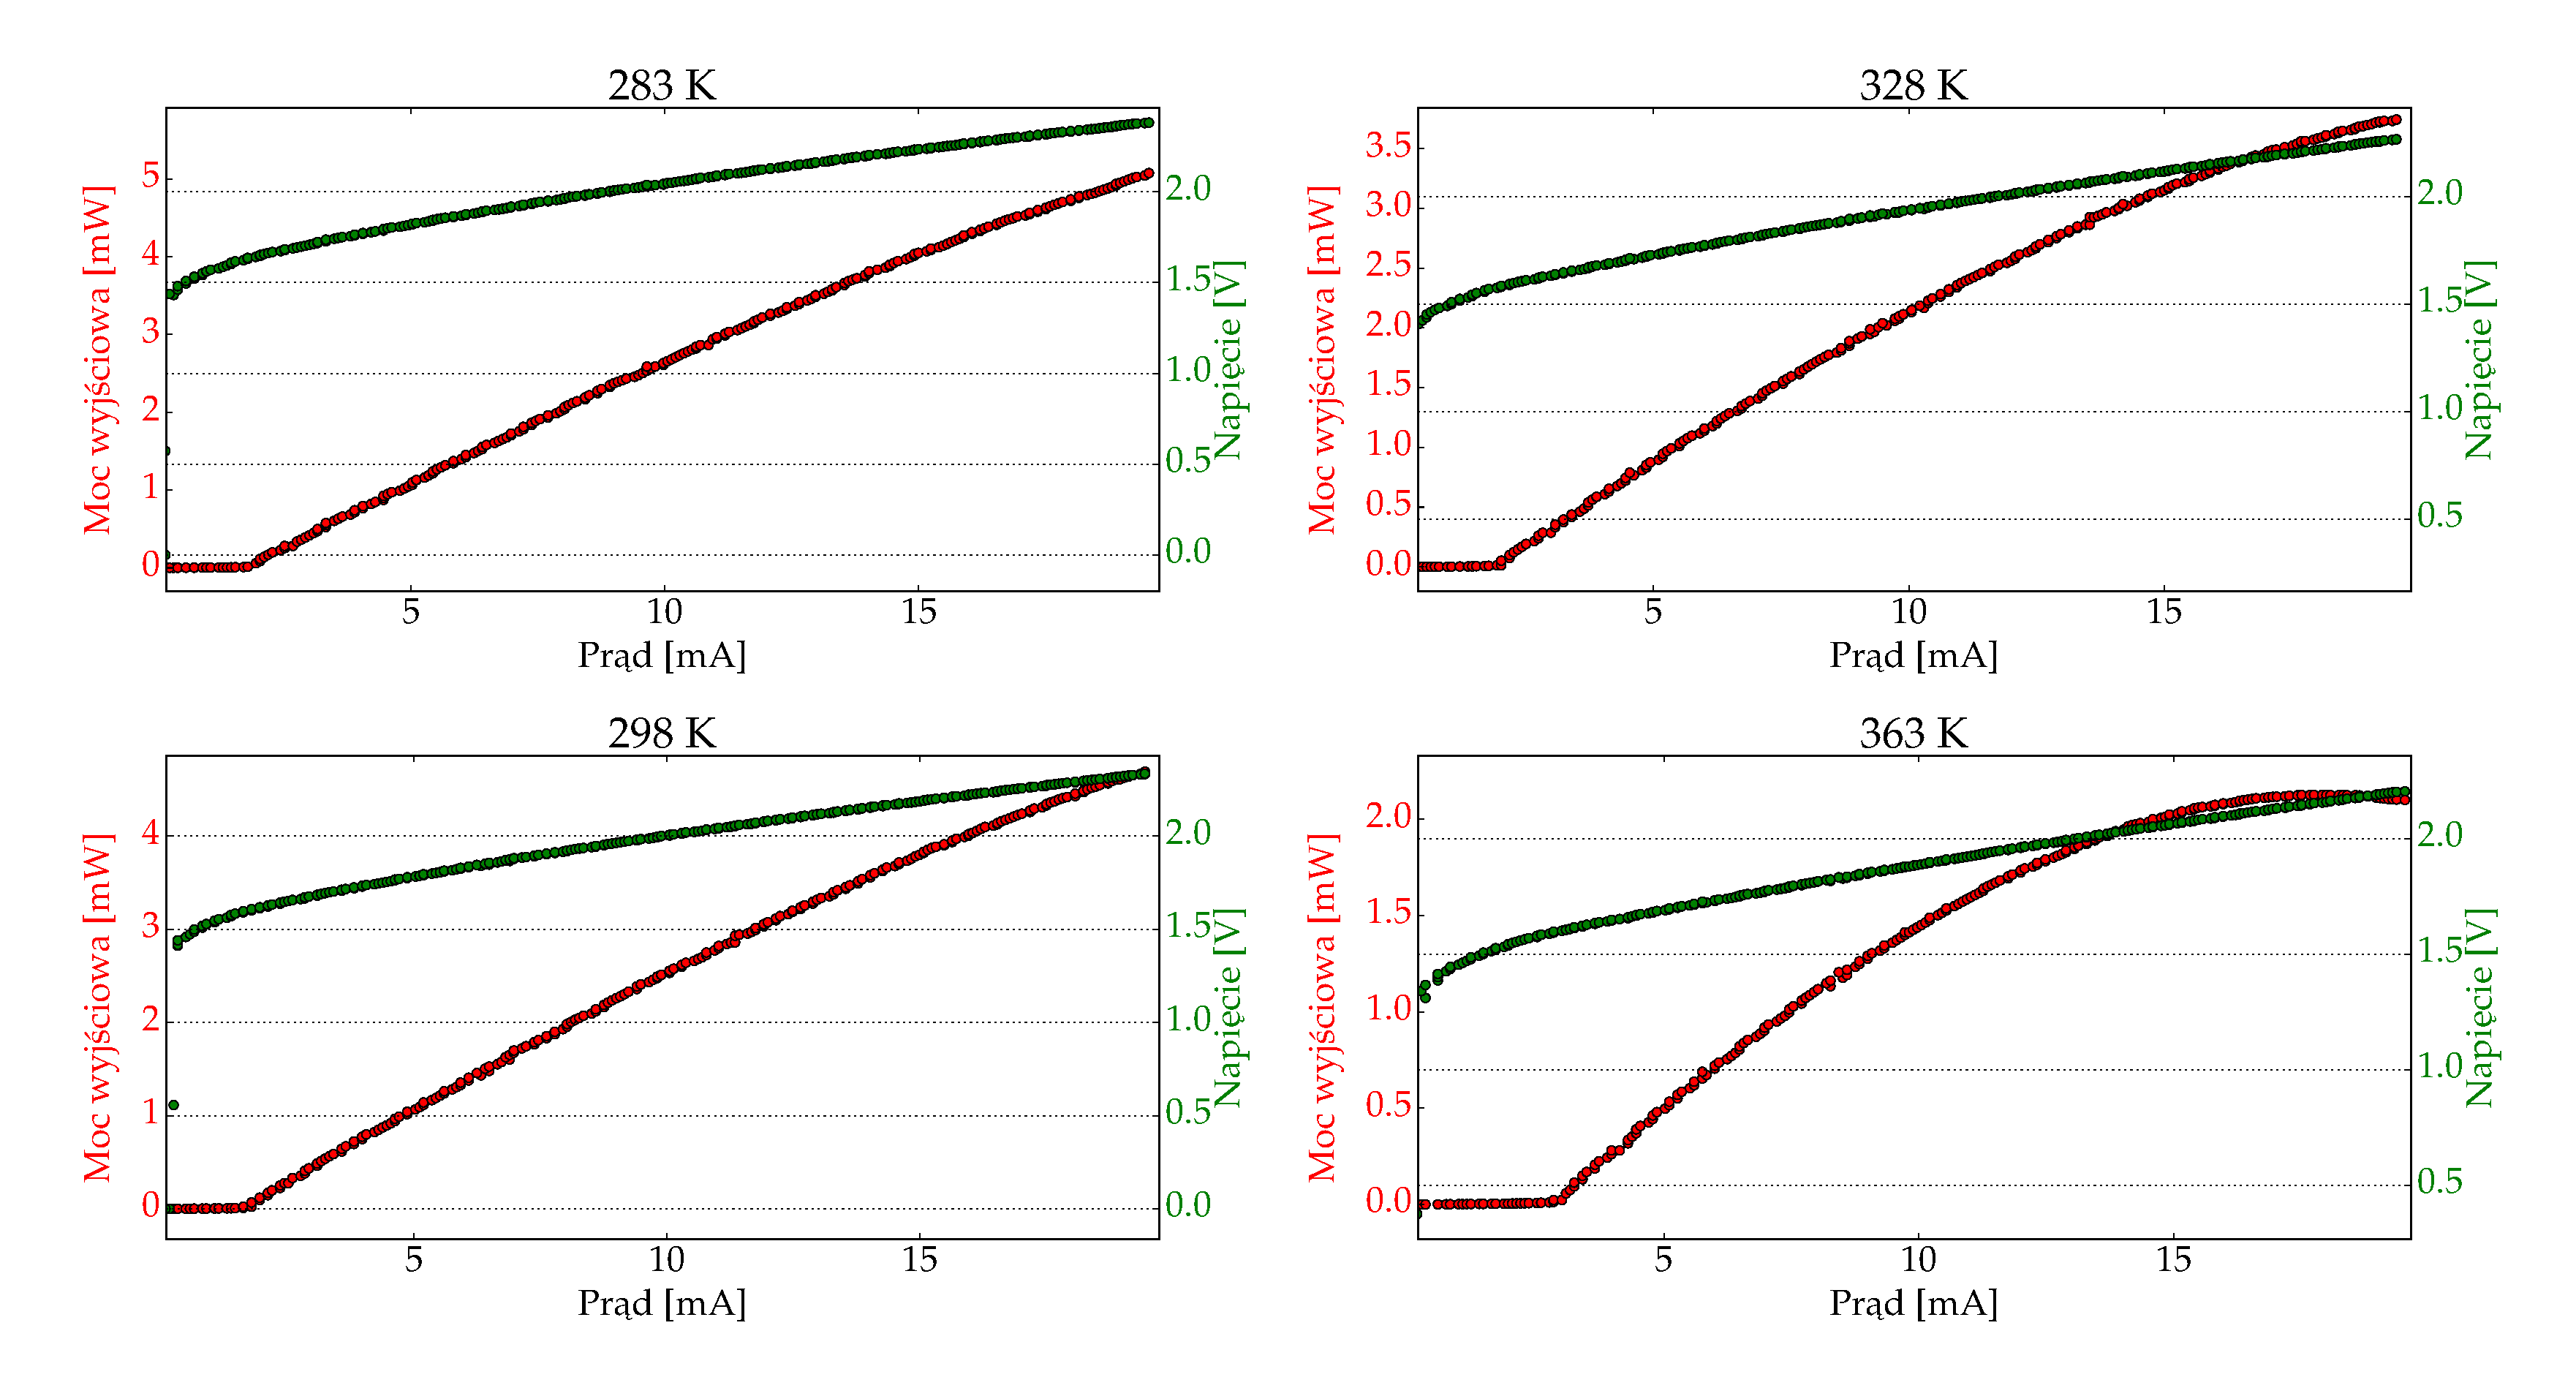
\includegraphics[scale=0.30]{plot635/plot_ivl_4.eps}
%  \label{rys1}
%  \caption{Wykres napięcia i mocy od prądu dla lasera krawędziowego 635\,nm.}
%\end{figure}
\begin{figure}[H]
\center
  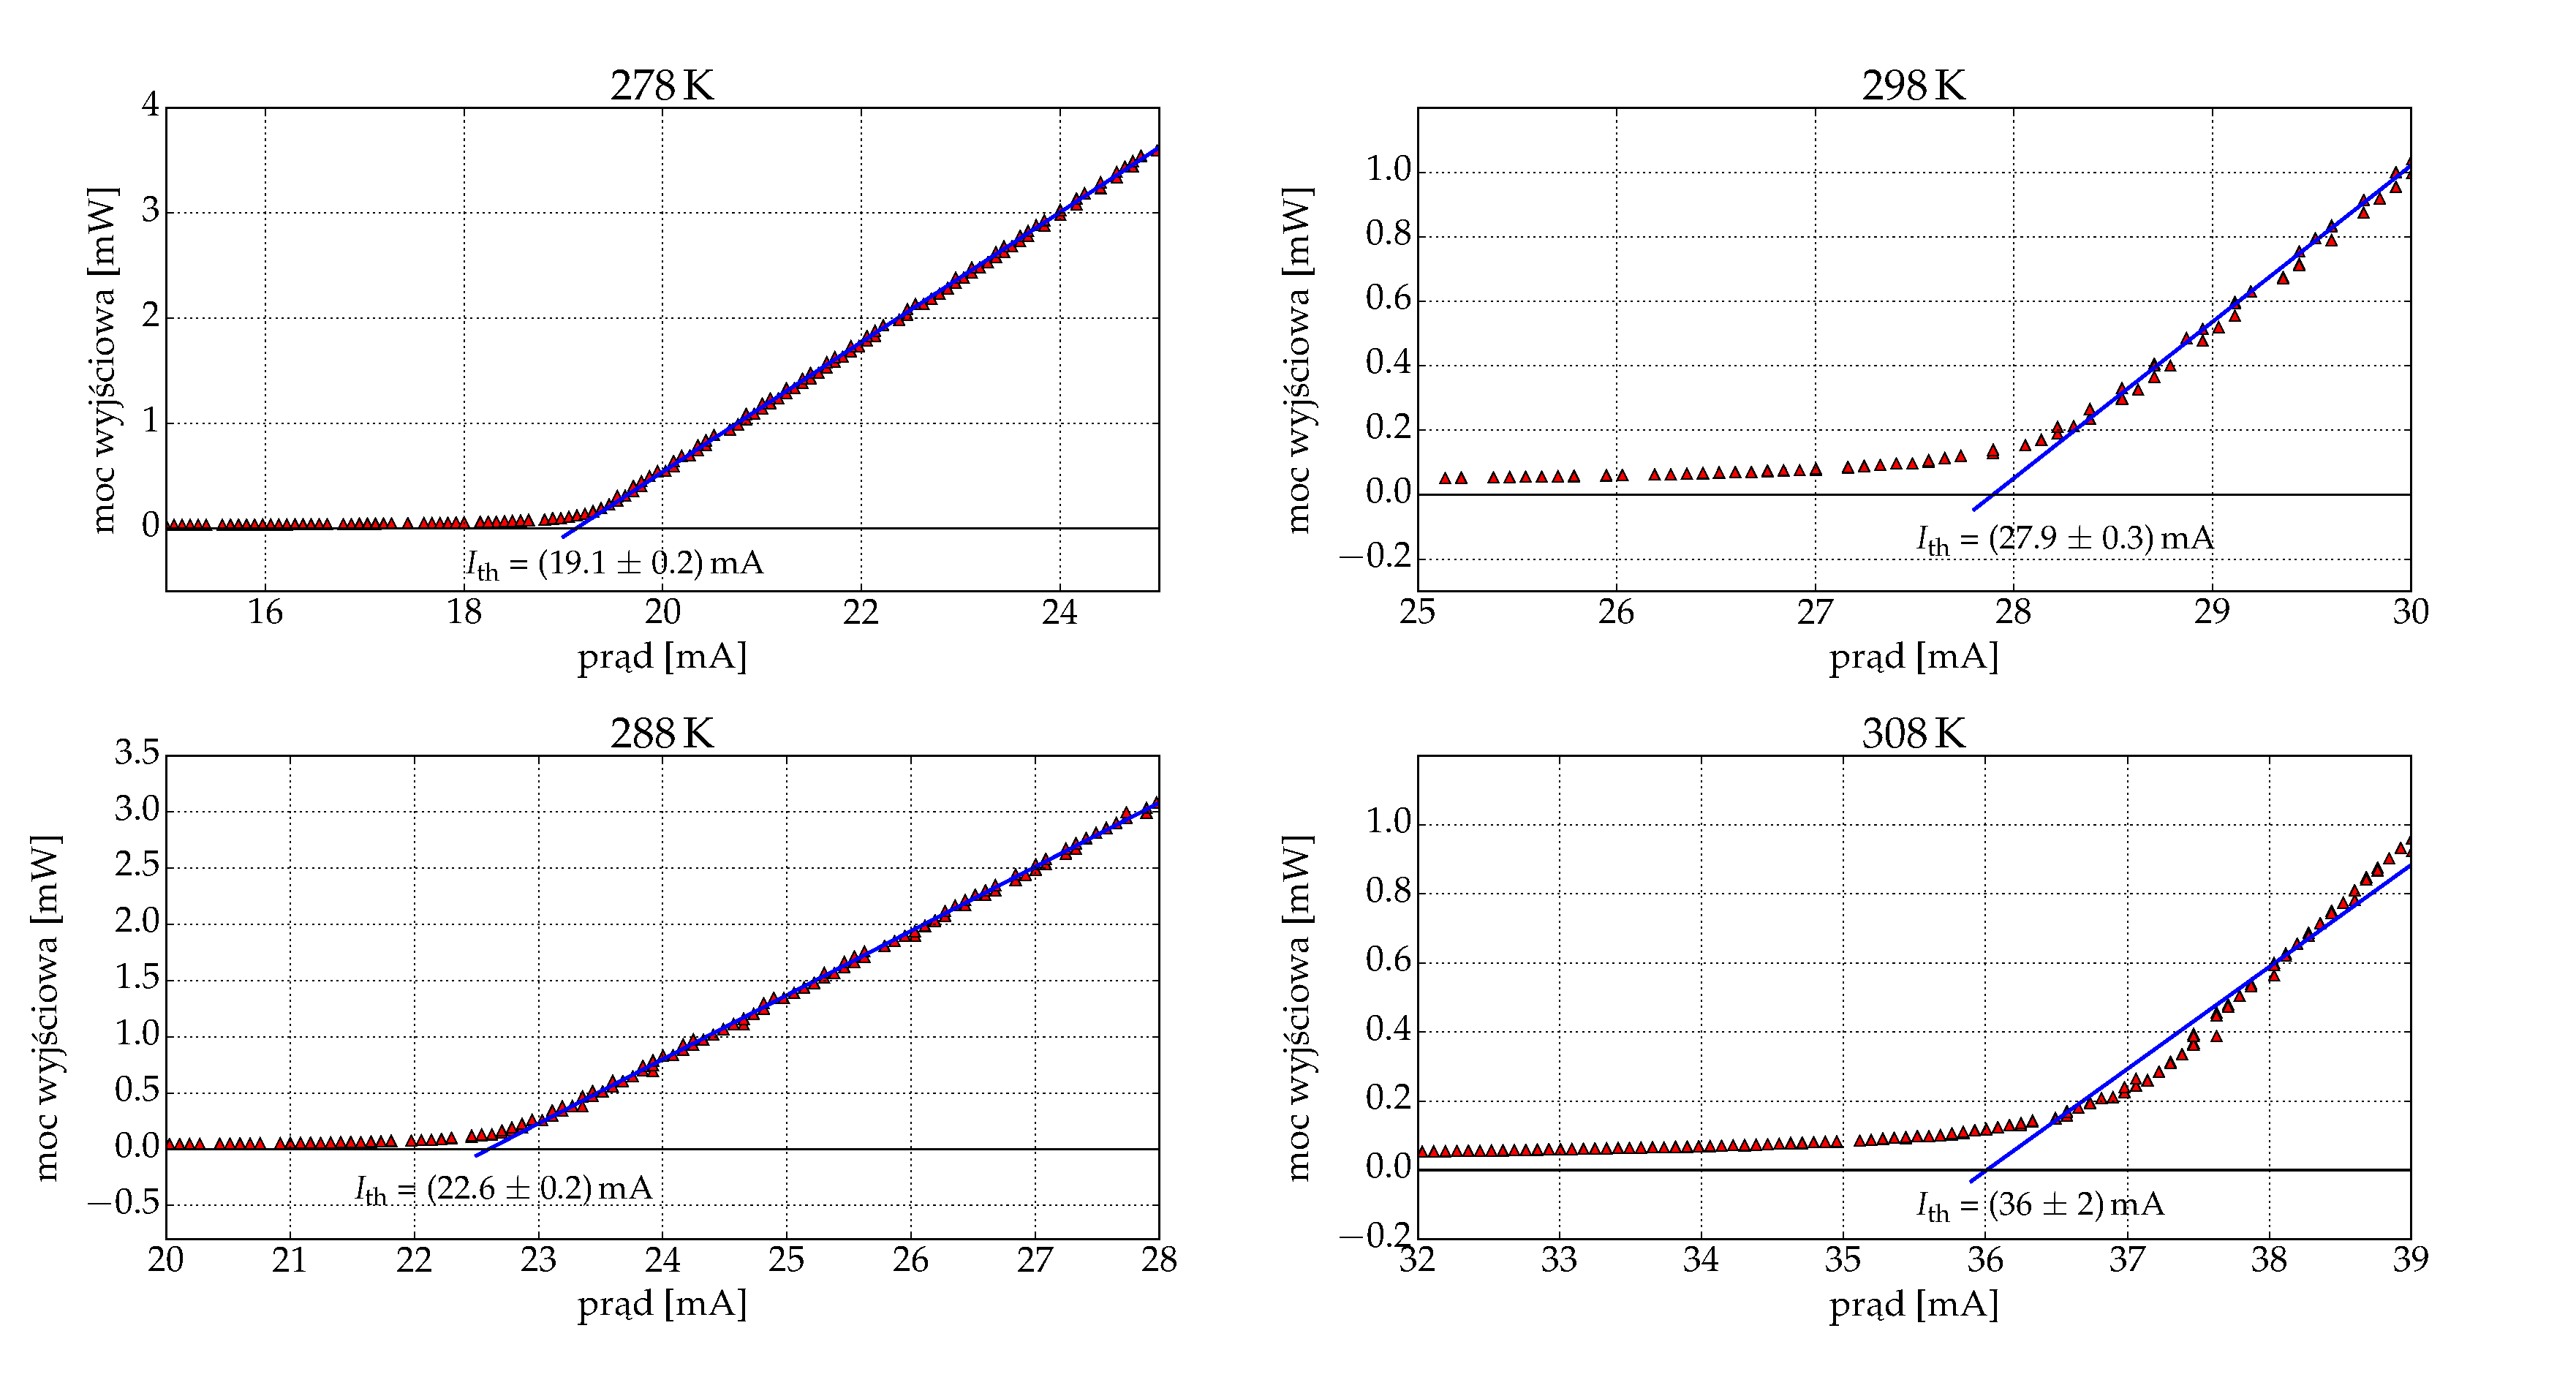
\includegraphics[scale=0.30]{plot635/plot_i_th_4.eps}
  \caption{Wykres ilustrujący wyznacznie prądu progowego dla lasera krawędziowego 635\,nm.}
  \label{fig:plot_i_th_4}
\end{figure}
\begin{figure}
\center
  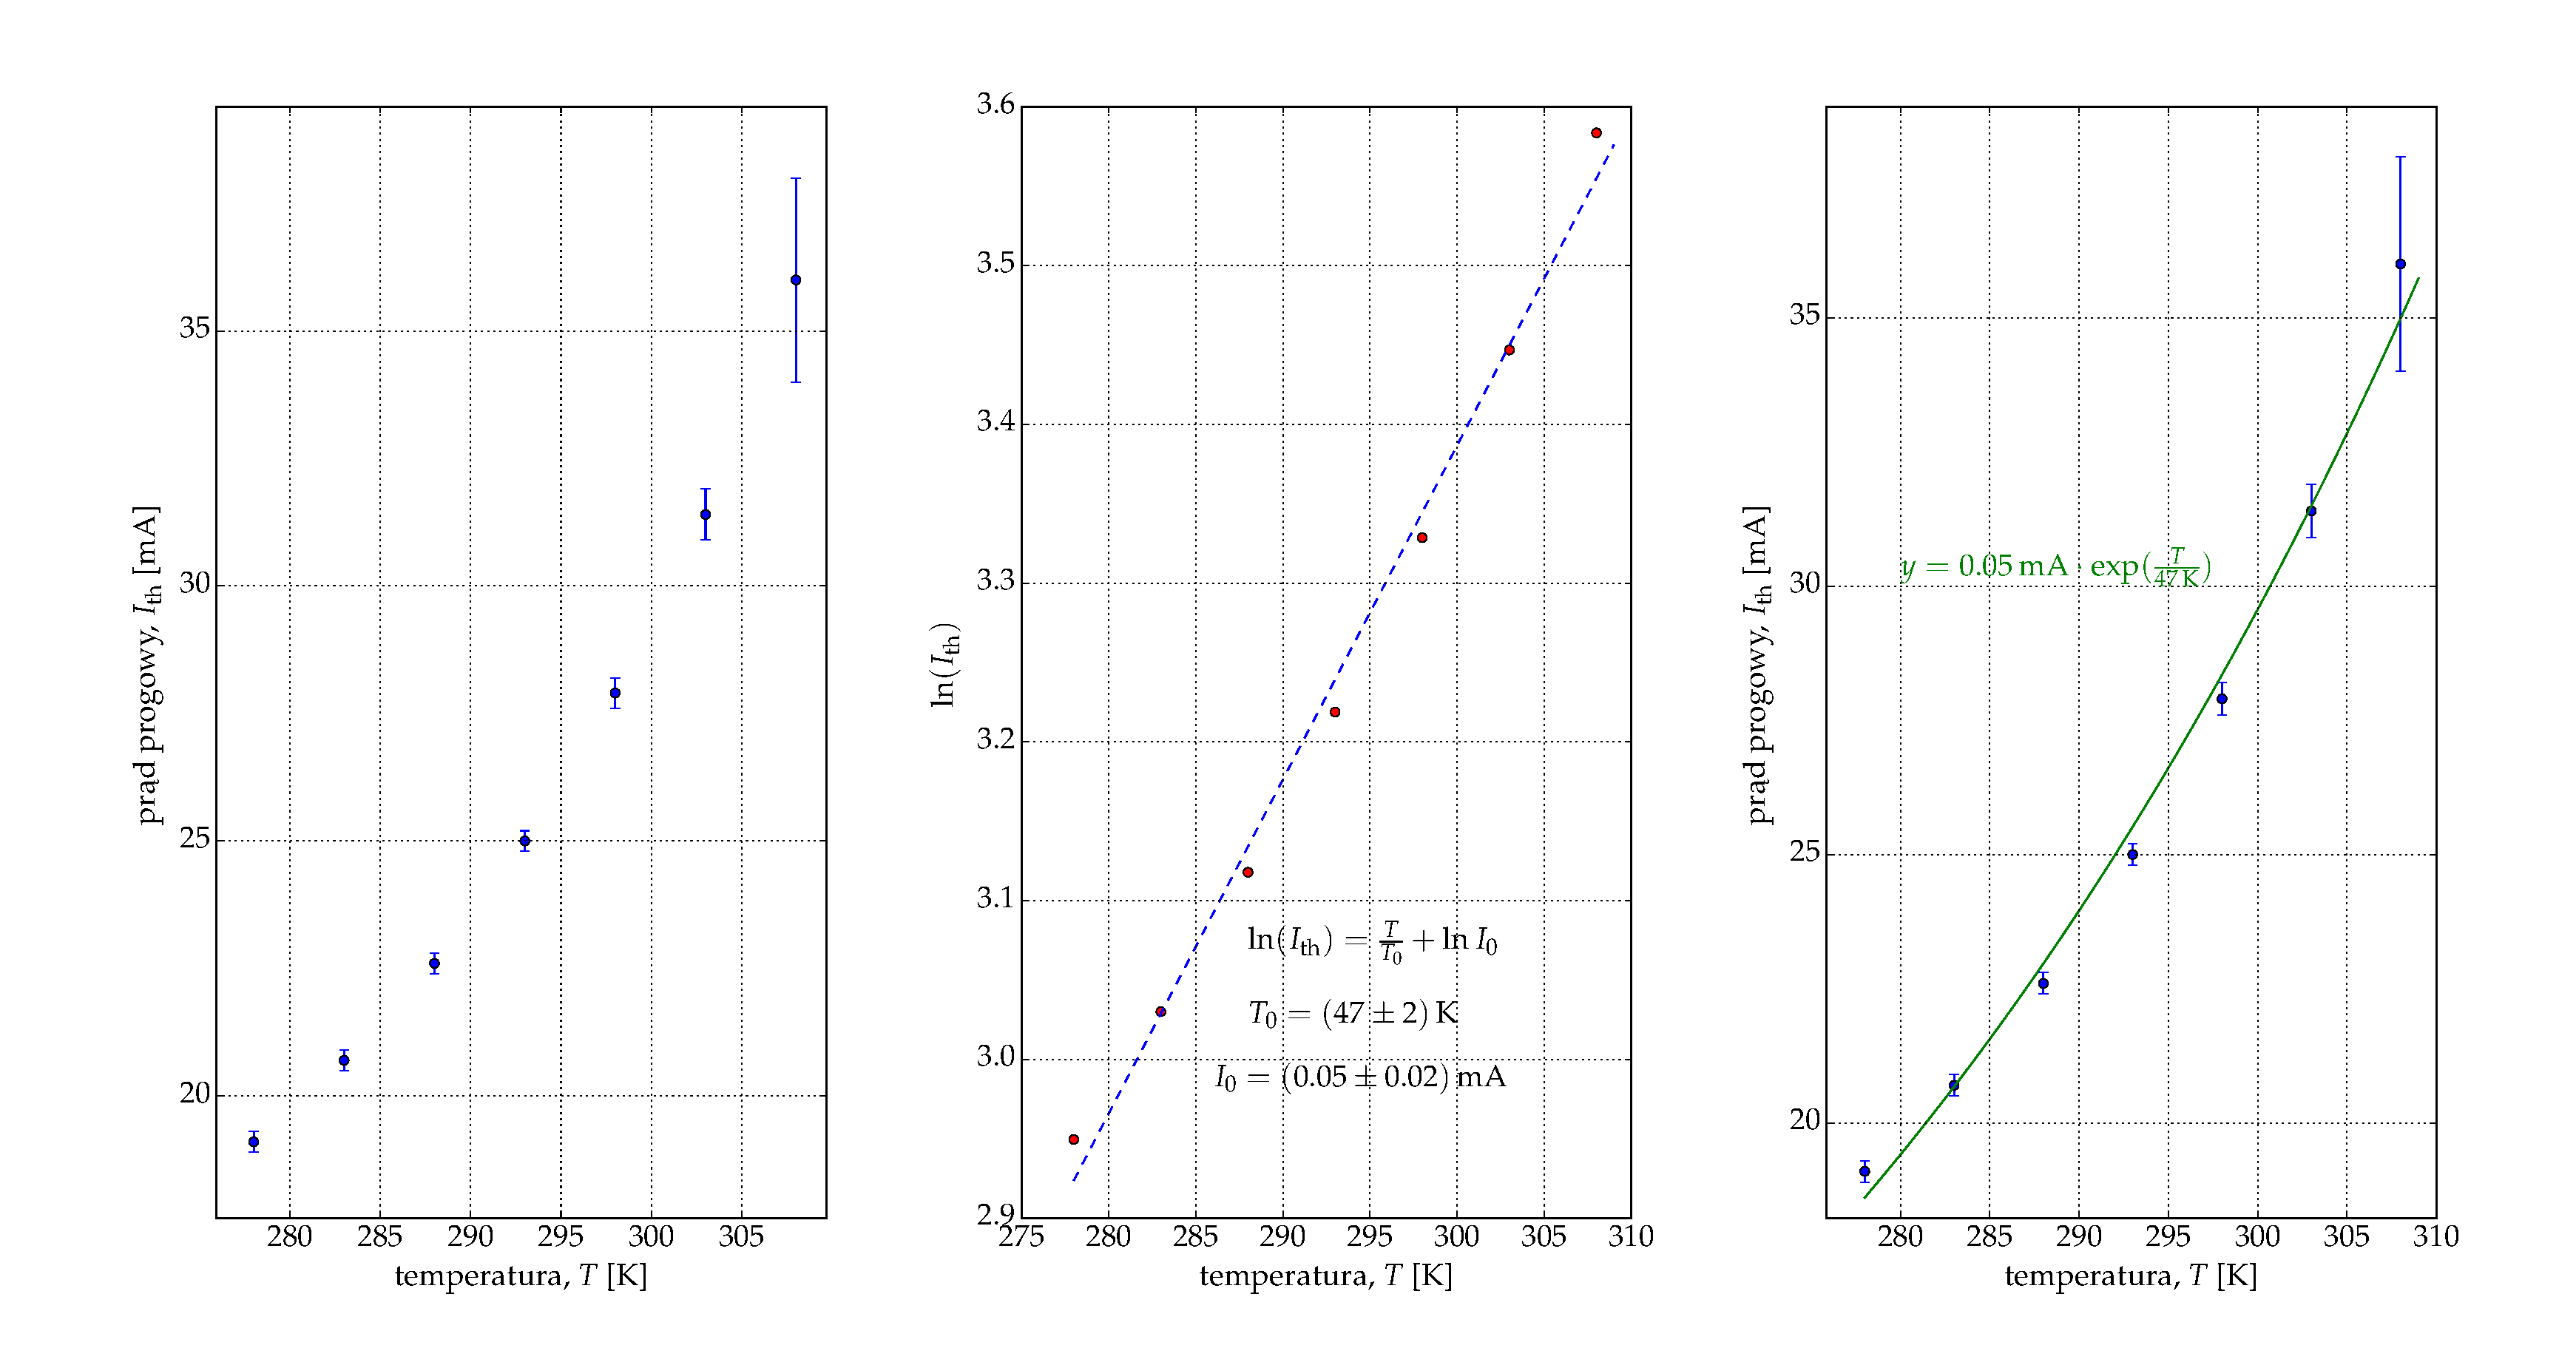
\includegraphics[scale=0.30]{plot635/plot_fit.eps}
  \caption{Wykres prądu progowego w zależności od temperatury chłodnicy z dopasowanymi wartościami $I_{0}$ i $T_{0}$ dla lasera krawędziowego 635\,nm.}
  \label{fig:plot_fit}
\end{figure}
\begin{figure}
\center
  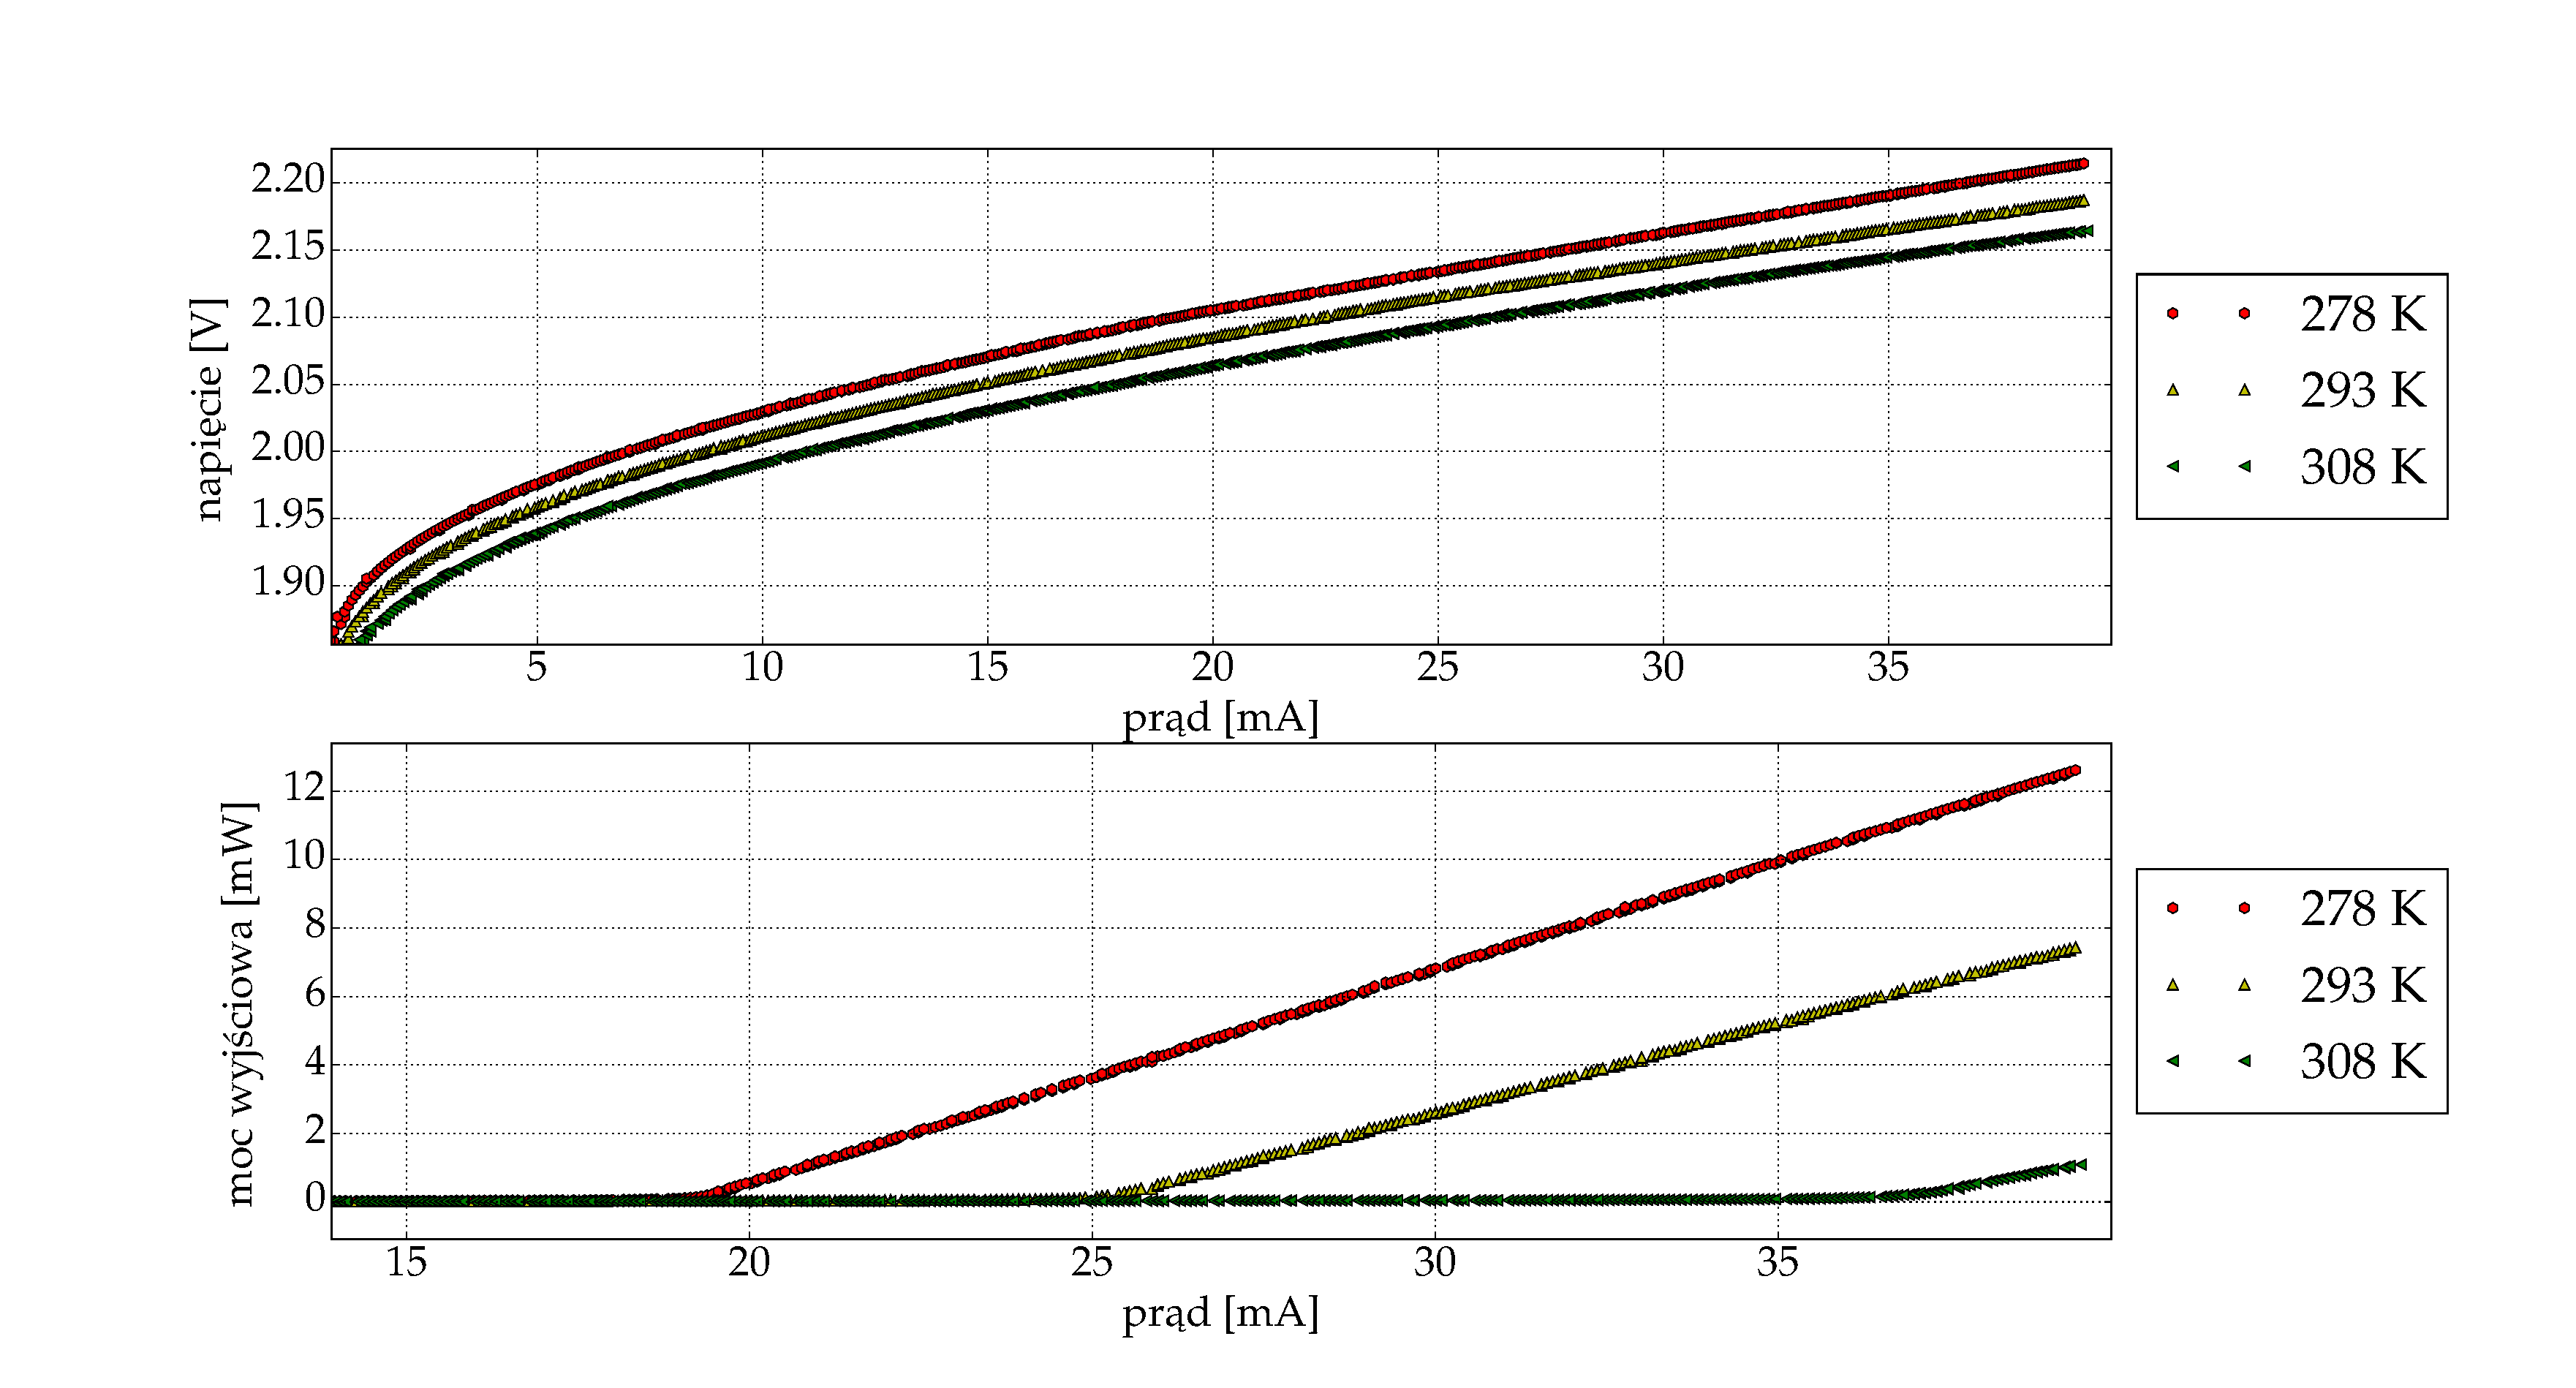
\includegraphics[scale=0.30]{plot635/plot_voltage_power.eps}
  \caption{Wykres napięcia na laserze oraz mocy w funkcji prądu dla lasera krawędziowego 635\,nm w trzech temperaturach.}
    \label{fig:plot_voltage_power_635}
\end{figure}
\begin{figure}
\center
  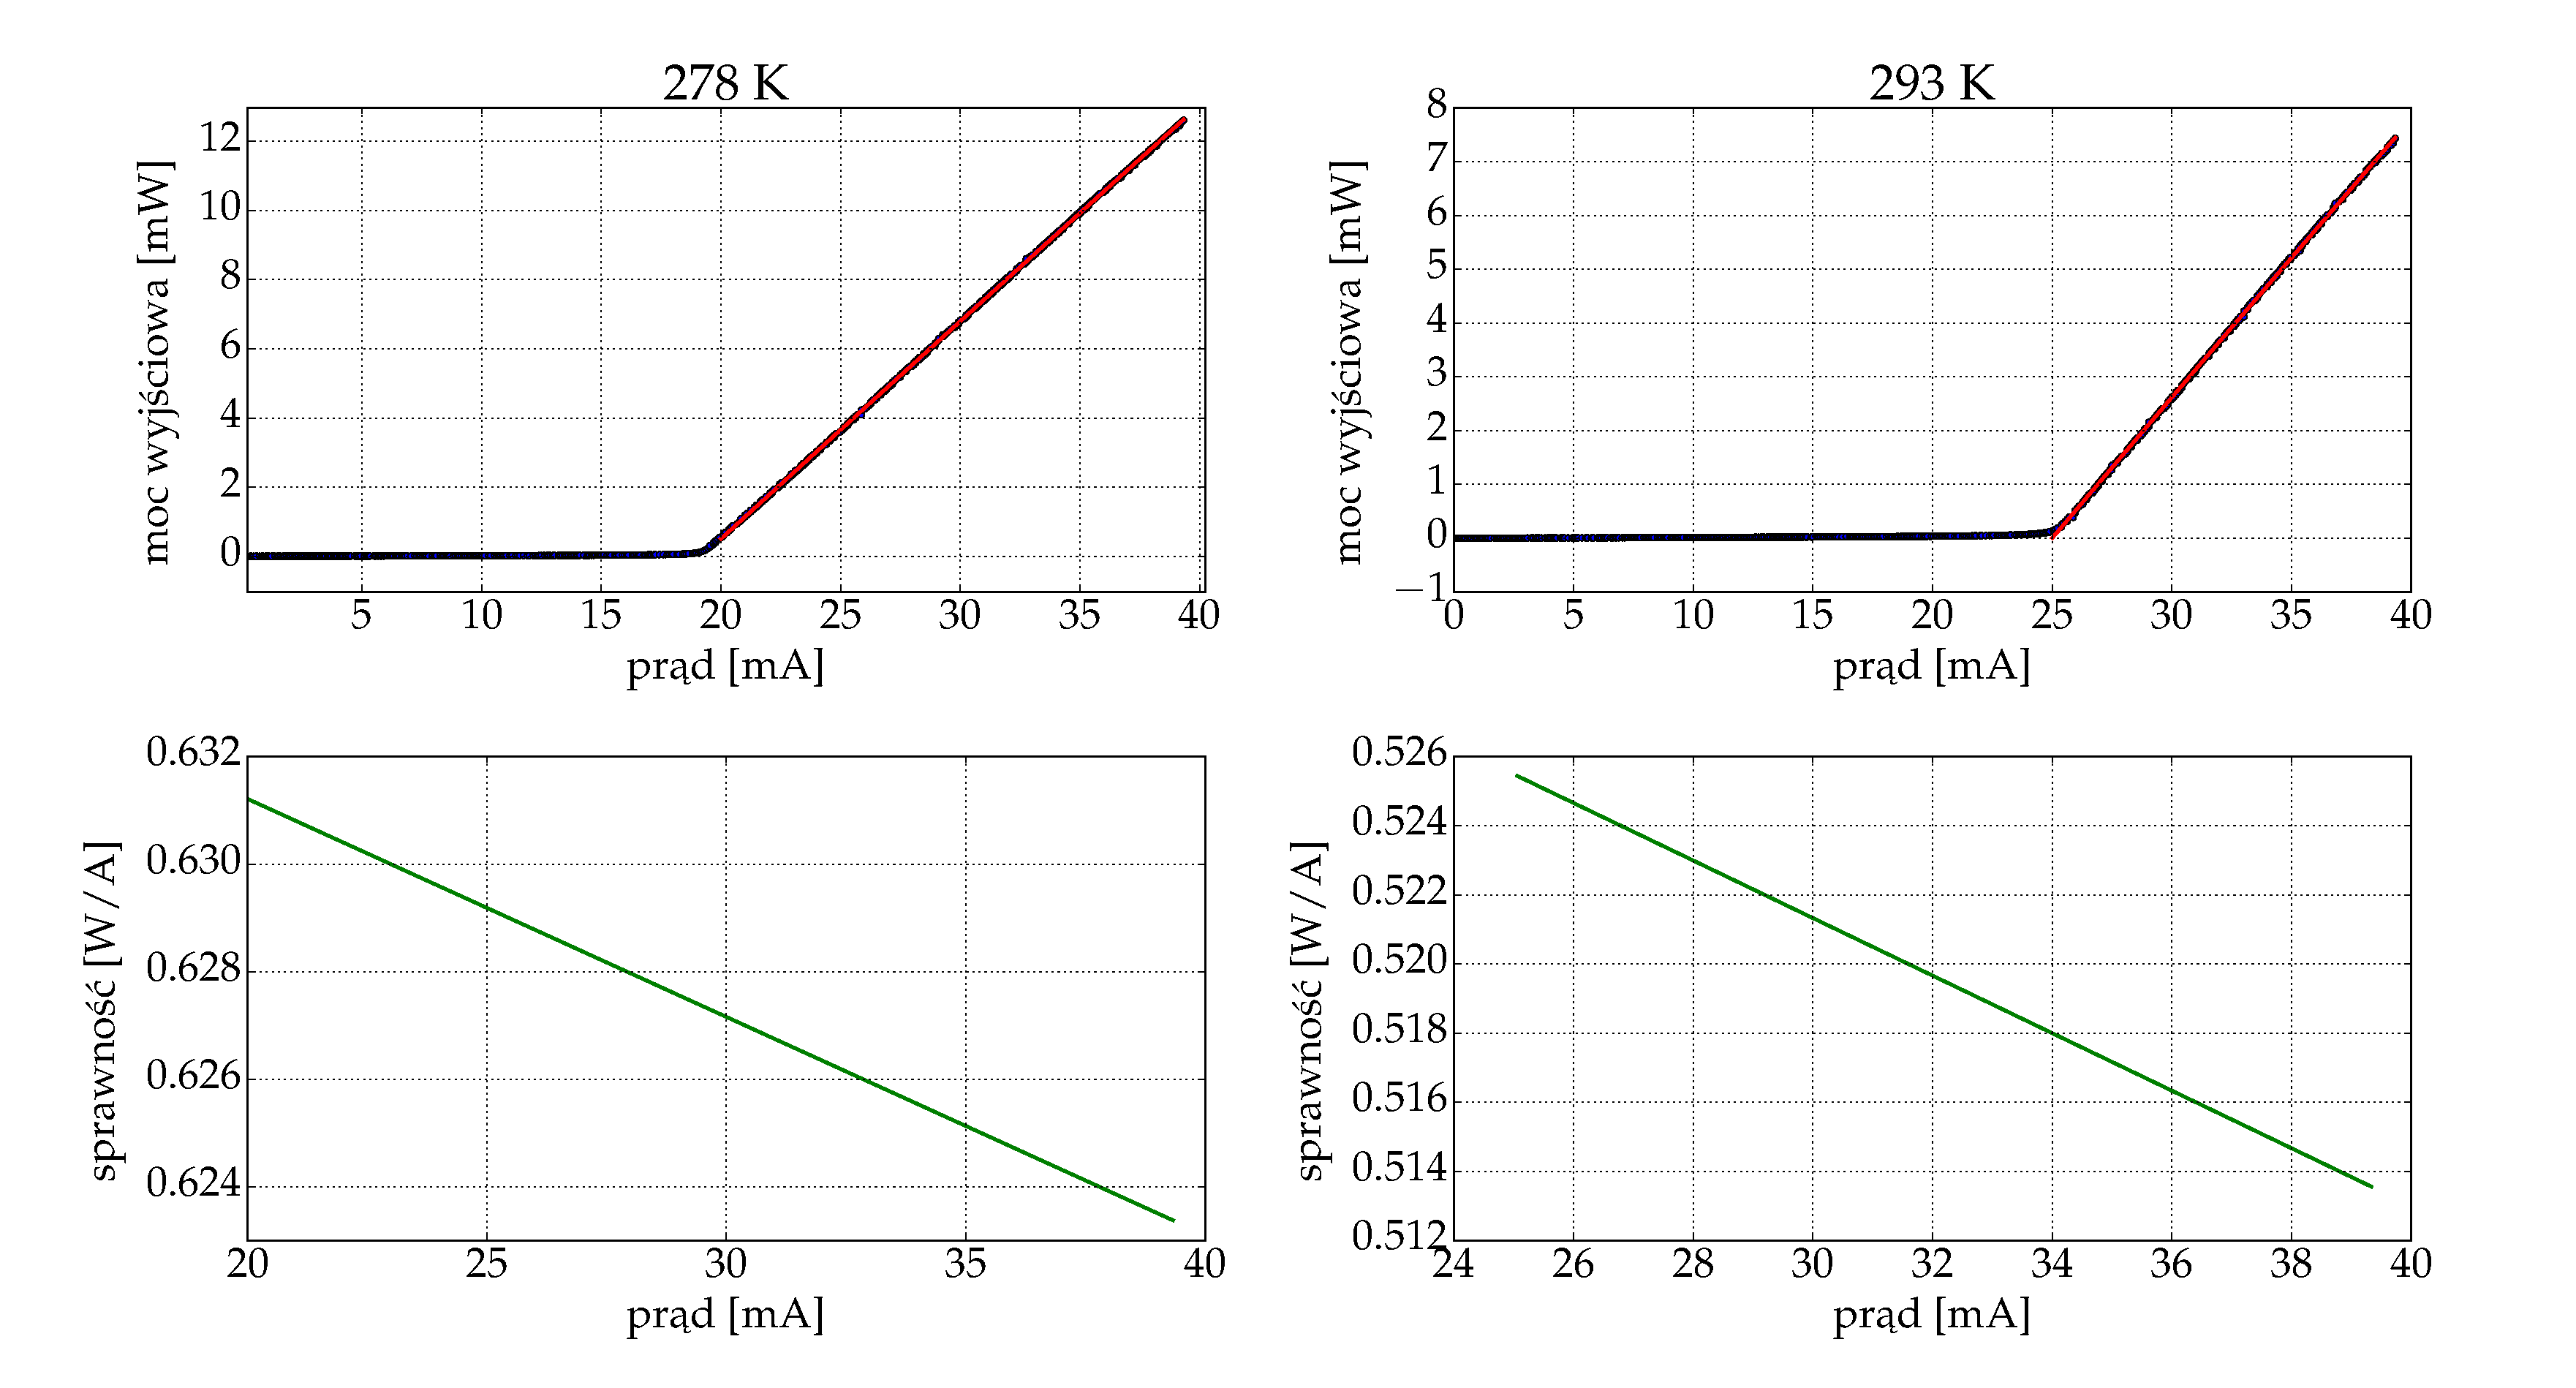
\includegraphics[scale=0.30]{plot635/plot_eff_via_current4.eps}
  \caption{Wykres sprawności różniczkowej dla lasera krawędziowego 635\,nm dla dwóch temperatur.}
  \label{fig:plot_eff_via_current4_635}
\end{figure}
\begin{figure}
\center
  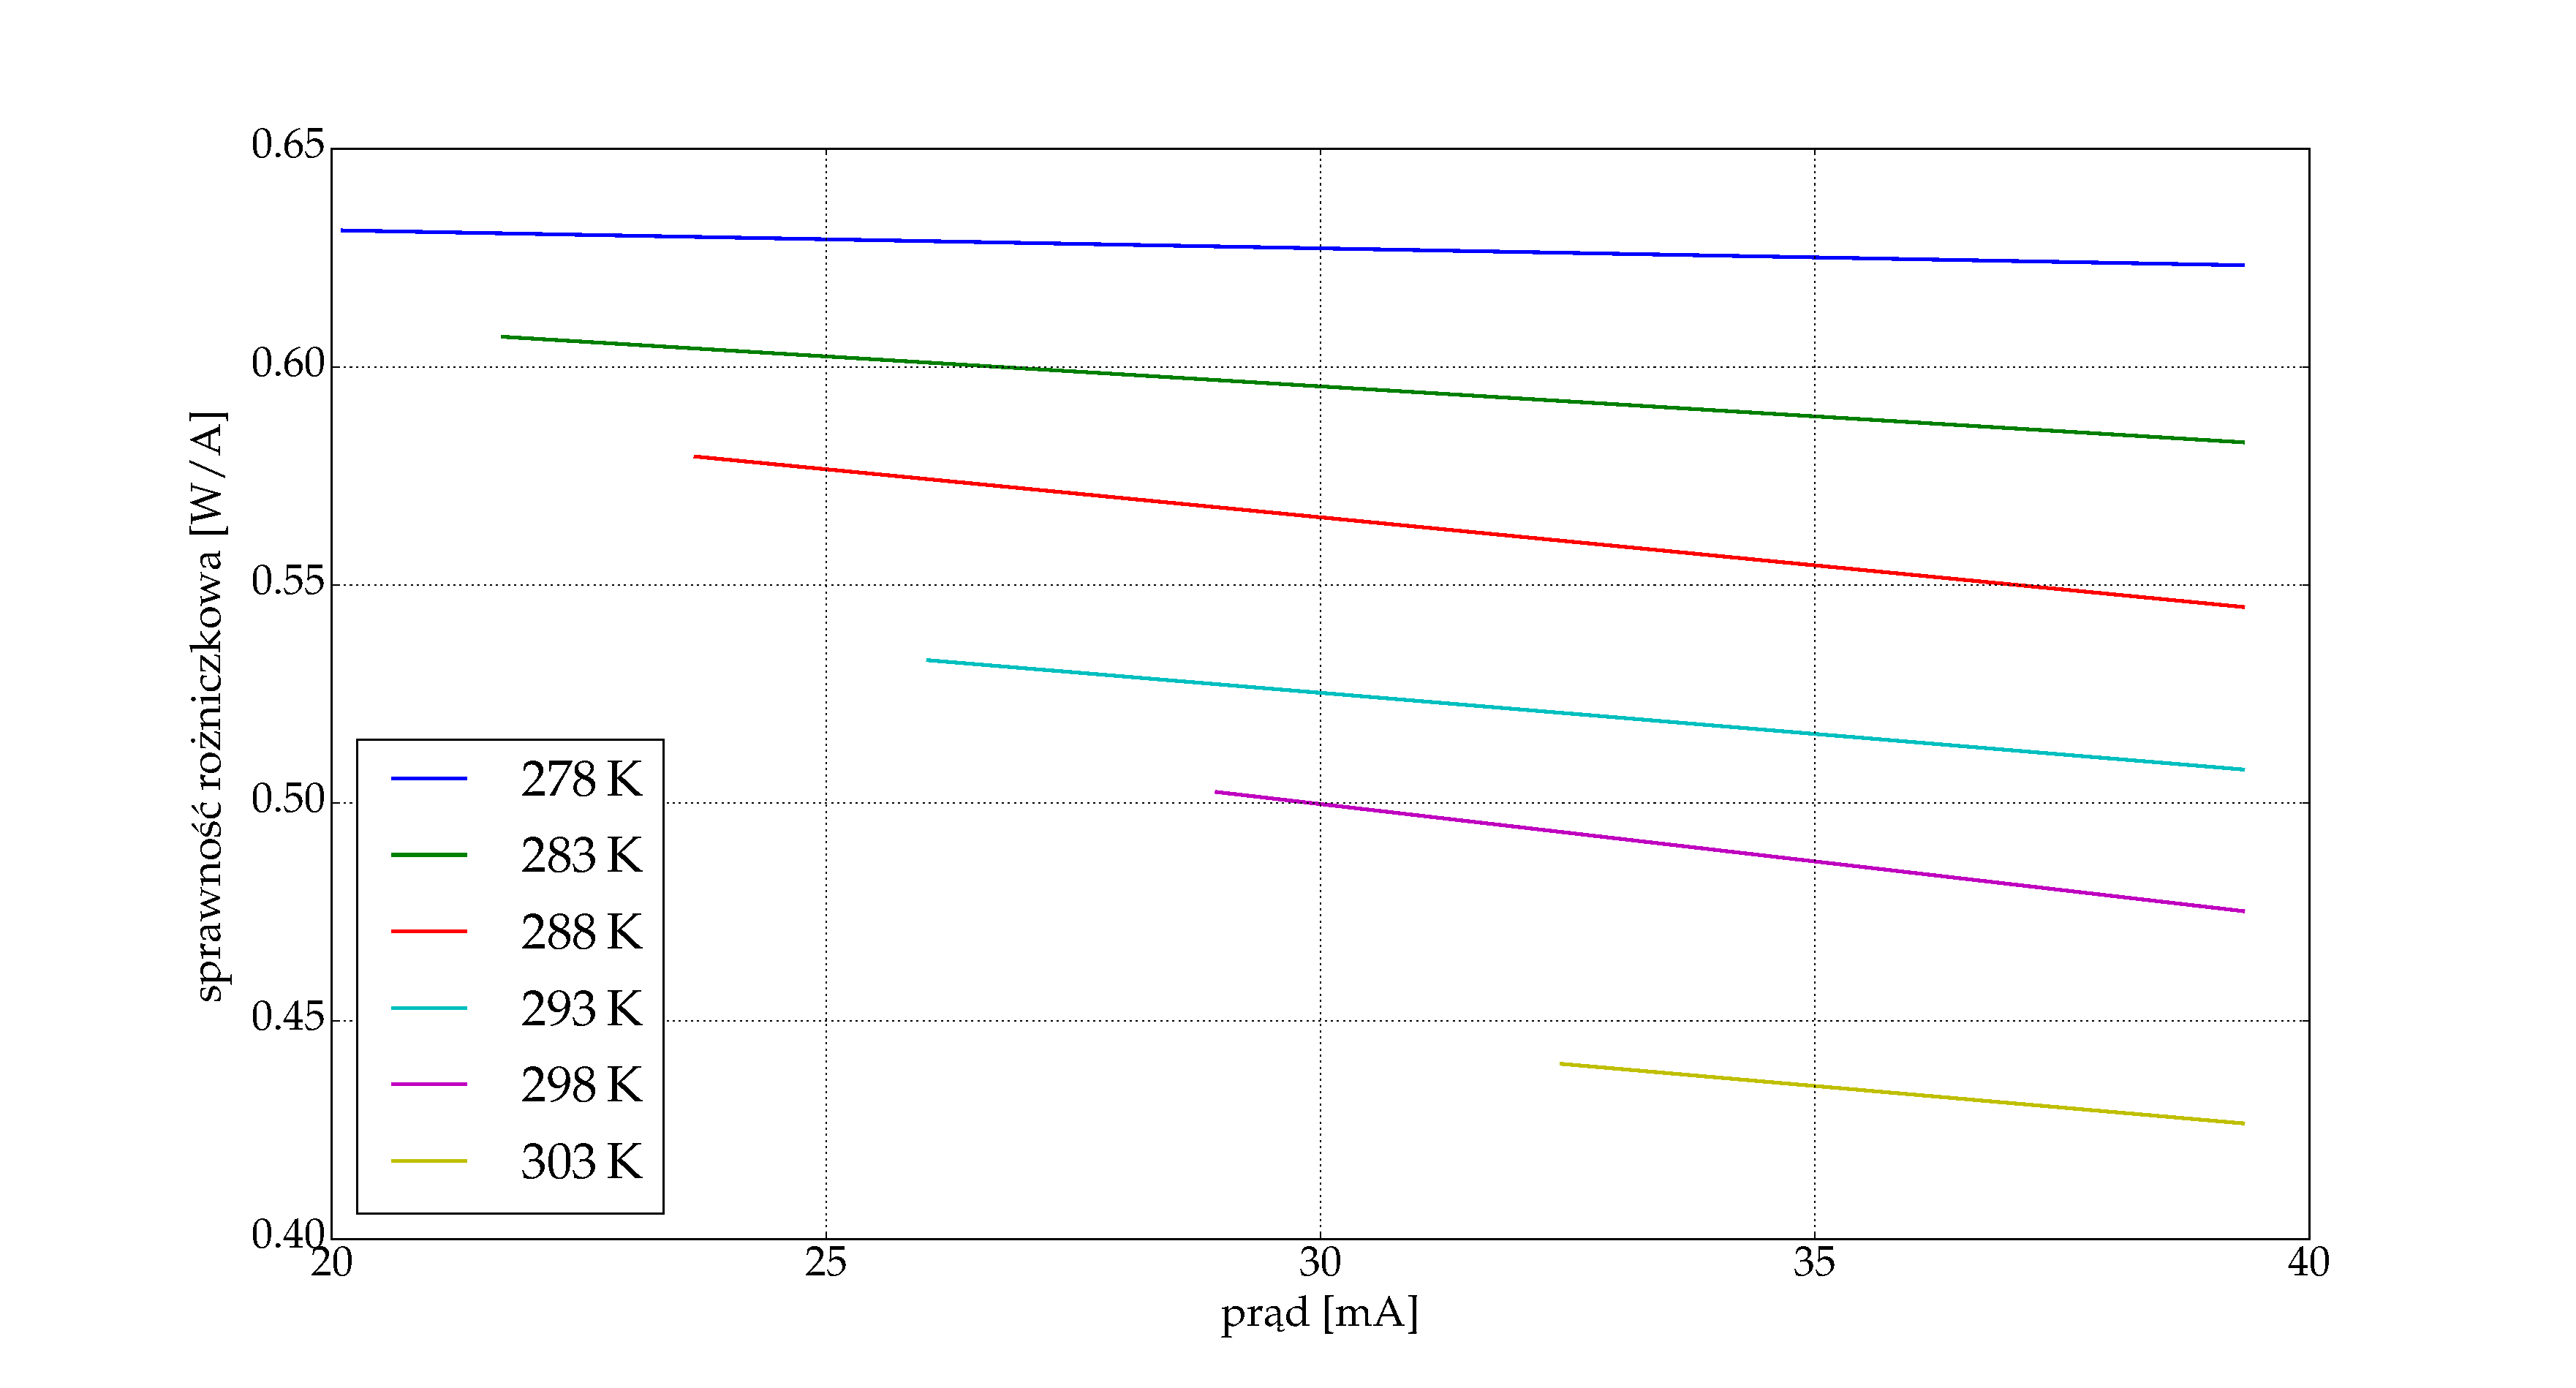
\includegraphics[scale=0.25]{plot635/plot_eff_via_current_all.eps}
  \caption{Wykres sprawności różniczkowej w funkcji prądu dla lasera krawędziowego 635\,nm.}
  \label{fig:plot_eff_via_current_all}
\end{figure}
\newpage
